\documentclass[a4paper]{beamer}
\usepackage[english]{babel}
\usepackage[utf8]{inputenc}
\usepackage{graphicx}
\usepackage{subcaption}
\usepackage{caption}
\usepackage{appendixnumberbeamer}
\usepackage{tikz}
\usepackage{csvsimple}
\usepackage{tabularx}
\usepackage{adjustbox}
\usepackage{pdfpages}

%\pgfpagesuselayout{resize to}[a4paper,border shrink=5mm,landscape]
\usepackage{cleveref}
\beamertemplatenavigationsymbolsempty
\usetheme{Boadilla}

\title[$H\gamma\gamma$ couplings]{Photon Energy Calibration Systematics}
\author[Goudet]{Christophe Goudet}
\institute[LAL]{\includegraphics[width=0.3\linewidth]{/home/goudet/Documents/LAL/ExternalPlot/LAL.jpg} }

\date{\today}

\begin{document}
\transboxin
\begin{frame}
\maketitle
\end{frame}

%%%=================================================================================
\begin{frame}{Methodology}
  \begin{minipage}{0.49\linewidth}
    For a given systematic source :
    \begin{itemize}
    \item Create distributions of \\ $m_{\gamma\gamma}^{nom}$, $m_{\gamma\gamma}^{up}$, $m_{\gamma \gamma}^{down}$
    \item Fit main parameter of the systematic with DSCB :
      \begin{itemize}
      \item Fit  $m_{\gamma\gamma}$
      \item Free parameter(s) of interest
      \item Fixing $X=\hat{X}^{nom}$
%        \item Fixing secondary parameter to nominal fitted values.
      \end{itemize}
      \item Systematic variation : $\delta_X=\frac{X^{fluct}}{X^{nom}}-1$, $X\in \{\mu , \sigma\}$
      \end{itemize}
    \end{minipage}
    \hfill
    \begin{minipage}{0.49\linewidth}
      \includegraphics[width=\linewidth]{plots/h013_EG_SCALE_ALL_0.pdf}
    \end{minipage}
    \vfill
    
    \begin{equation}
      \tiny
      CB(m_{\gamma \gamma}) = 
      \begin{cases}
        e^{-t^{2}/2} & \text{if } -\alpha_{low} \leq t \leq \alpha_{high} \\
        \frac{ e^{-{}^{1}_{2} \alpha_{low}^{2}} } { \left[ \frac{1}{R_{low}} \left(R_{low} - \alpha_{low} - t \right) \right]^{n_{low}} } & \text{if } t < -\alpha_{low} \\
        \frac{ e^{-{}^{1}_{2} \alpha_{high}^{2}} } { \left[ \frac{1}{R_{high}} \left(R_{high} - \alpha_{high} + t \right) \right]^{n_{high}} } & \text{if } t > \alpha_{high} \\
        t=(m_{\gamma\gamma}-\mu)/\sigma, R_{low}=\frac{\alpha_{low}}{n_{low}},  R_{high}=\frac{\alpha_{high}}{n_{high}} \\
      \end{cases}
    \end{equation}
\end{frame}
%%=================================================================================
\begin{frame}{ICHEP Results}
  \begin{minipage}{0.59\linewidth}
    ICHEP results were obtained with only 2 nuisance parameters.\\
    %    \textcolor{red}{Only the fluctuation effects on the POI were considered for the measurement framework.}
    \textcolor{red}{In stat framework, systematic only affects a single dedicated parameter (width or mass).}\\
    \input{plots/h013_ICHEP_PhotonSyst.csv}
    \vfill
  \end{minipage}
  \begin{minipage}{0.4\linewidth}
    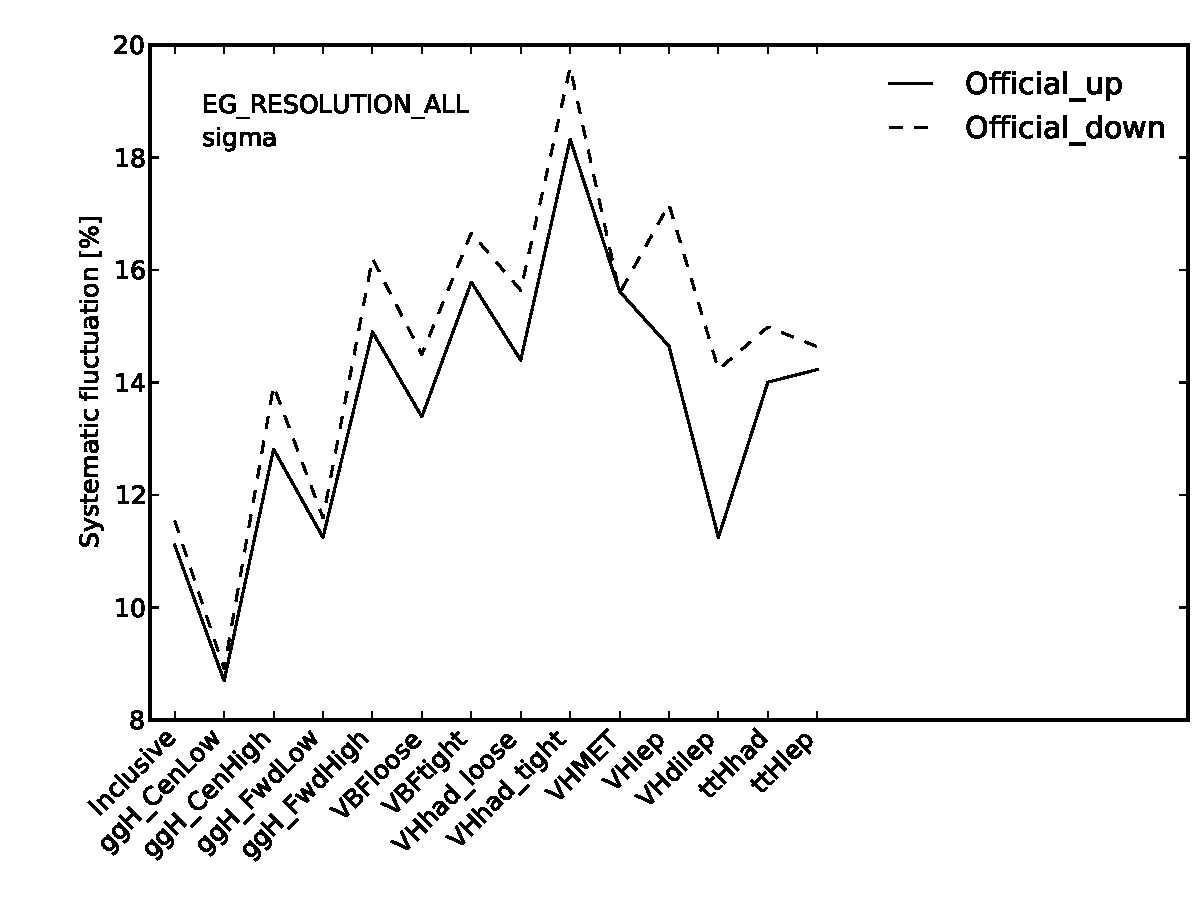
\includegraphics[width=\linewidth]{plots/h013_ICHEP_PhotonSyst_EG_RESOLUTION_ALL_sigma.pdf}\\
    \includegraphics[width=\linewidth]{plots/h013_ICHEP_PhotonSyst_EG_SCALE_ALL_mean.pdf}\\
  \end{minipage}
\end{frame}

\begin{frame}{Calibration uncertainties contributions}
  \begin{minipage}{0.49\linewidth}
    \includegraphics[width=\linewidth]{/home/goudet/Documents/LAL/ExternalPlot/ATL-COM-PHYS-2016-222_74f.pdf}\\
    \centering
    ATL-COM-PHYS-2016-222
  \end{minipage}
  \begin{minipage}{0.49\linewidth}
    \begin{itemize}
    \item \textcolor{red}{Resolution systematic dominant}
    \item Consequent other experimental contribution
    \item Energy scale has small contribution
    \end{itemize}
  \end{minipage}
\end{frame}

%==============================================================================
\begin{frame}{Cross-check : template method}
\begin{minipage}{0.59\linewidth}
  The template method is used to measure $\alpha$ and $C$ simultaneously.
\begin{itemize}
\item Create distorded MC (templates) with test values of $\alpha$ and $C$.
\item \textcolor{blue}{\bf Compute $\chi^2$ between Z mass distribution of data and template}.
\item \textcolor{blue}{\bf Fit the minimum of the $\chi^2$ distribution} in the ($\alpha,C$) plane.
\item Fit performed in 2 steps of 1D fits : 
\begin{itemize}
\item fit $\chi^2=f(\alpha)$ at constant $C$ (lines) $\rightarrow (\alpha_{min}, \chi^2_{min})$ .
\item fit $\chi^2_{min}=f(C)\rightarrow (C, \Delta C)$
\item project $C$ in $\alpha_{min}=f(C)$, corresponding bin gives $(\alpha, \Delta\alpha)$.
\end{itemize}
\end{itemize}
  \includegraphics[width=0.325\linewidth]{/home/goudet/Documents/LAL/Slides/Archive/Method/plot/MC6_0_0_chi2FitNonConstVar_10.pdf}
  \includegraphics[width=0.325\linewidth]{/home/goudet/Documents/LAL/Slides/Archive/Method/plot/MC6_0_0_chi2FitConstVar.pdf}
  \includegraphics[width=0.325\linewidth]{/home/goudet/Documents/LAL/Slides/Archive/Method/plot/MC6_0_0_corAngle.pdf}
\end{minipage}
\hfill
\begin{minipage}{0.4\linewidth}
  \includegraphics[width=\linewidth]{/home/goudet/Documents/LAL/Slides/Archive/Method/plot/MC6_0_0_CompareAlpha.pdf}\\
  \includegraphics[width=\linewidth]{/home/goudet/Documents/LAL/Slides/Archive/Method/plot/MC6_0_0_chiMatrix.pdf}\\
\end{minipage}
\end{frame}

%==============================================================================
\begin{frame}{Scale factors interpretation}
  \begin{minipage}{0.49\linewidth}
    Assume the up fluctuation (red) as data and nominal distribution (black) as MC in the template method.
    One has
    $$m_H^{up}=m_H^{nom}(1+\alpha)$$
    Hence
    $$\delta_{m_H}=\alpha$$
    \end{minipage}
  \begin{minipage}{0.49\linewidth}
    \includegraphics[width=\linewidth]{plots/h013_EG_SCALE_ALL_0.pdf}
  \end{minipage}
  Furthermore :
  $$\sigma_H^{up}=\sigma_H^{nom} \oplus cE$$
  Hence
  $$\delta_{\sigma_H} = \sqrt{1+\frac{c^2E^2}{\sigma_H^2}}-1$$
  One has to be carefull with resolution uncertainty as the template method is weak to measure small differences.
\end{frame}


%%=================================================================================
\begin{frame}{Model Comparison}
    Two correlation models of systematics are proposed : 
  \begin{itemize}
  \item FULL model decorrelate all NP.
  \item ALL model sum in quadrature respectively all systematic sources into respectively a single nuisance parameter for scale and resolution.
  \item The fit with $m_{\gamma\gamma}\in[115,135]$GeV is used as closest to the signal model tool default behaviour.
  \item Major (surprising?) difference for scale uncertainty
  \end{itemize}
  \begin{center}
    Total Inclusive Uncertainty :\\
    \begin{tabular}{l|rr}
      \% & Scale & Resolution \\
      \hline
      FULL & 0.27 & 8.26 \\
      ALL & 0.46 & 9.02 \\
    \end{tabular}
  \end{center}
\end{frame}

%==================================================
\begin{frame}{Exact uncertainty}
  (Thanks Guillaume for explanation)
  \begin{itemize}
  \item Consider $N_{NP}$ NP with constant values $N_B$ bins (in $\eta$, $p_T$, conversion status).
  \item The covariance matrix $V$ is then defined as :
    \begin{equation}
      V_{ij} = \sum\limits_{n}^{N_{NP}} \sigma_{n,i}\sigma_{n,j}
    \end{equation}
  \item The total inclusive uncertainty on measured mass is then, 
    \begin{equation}
      \frac{\sigma_M}{M} = \frac{1}{N_\gamma}\sqrt{\sum\limits_{ij}^{N_B} N_iN_jV_{ij}}
    \end{equation}
    $N_i$ = number of photons in bin $i$,
    
  \end{itemize}
\end{frame}
%==================================================
\begin{frame}{Models total mass uncertainty}
  (Thanks Guillaume for cross-check)
  
  \centering
  \begin{minipage}{0.49\linewidth}\centering ALL \end{minipage}
  \hfill
  \begin{minipage}{0.49\linewidth}\centering FULL \end{minipage}

  Correlation matrix\\
  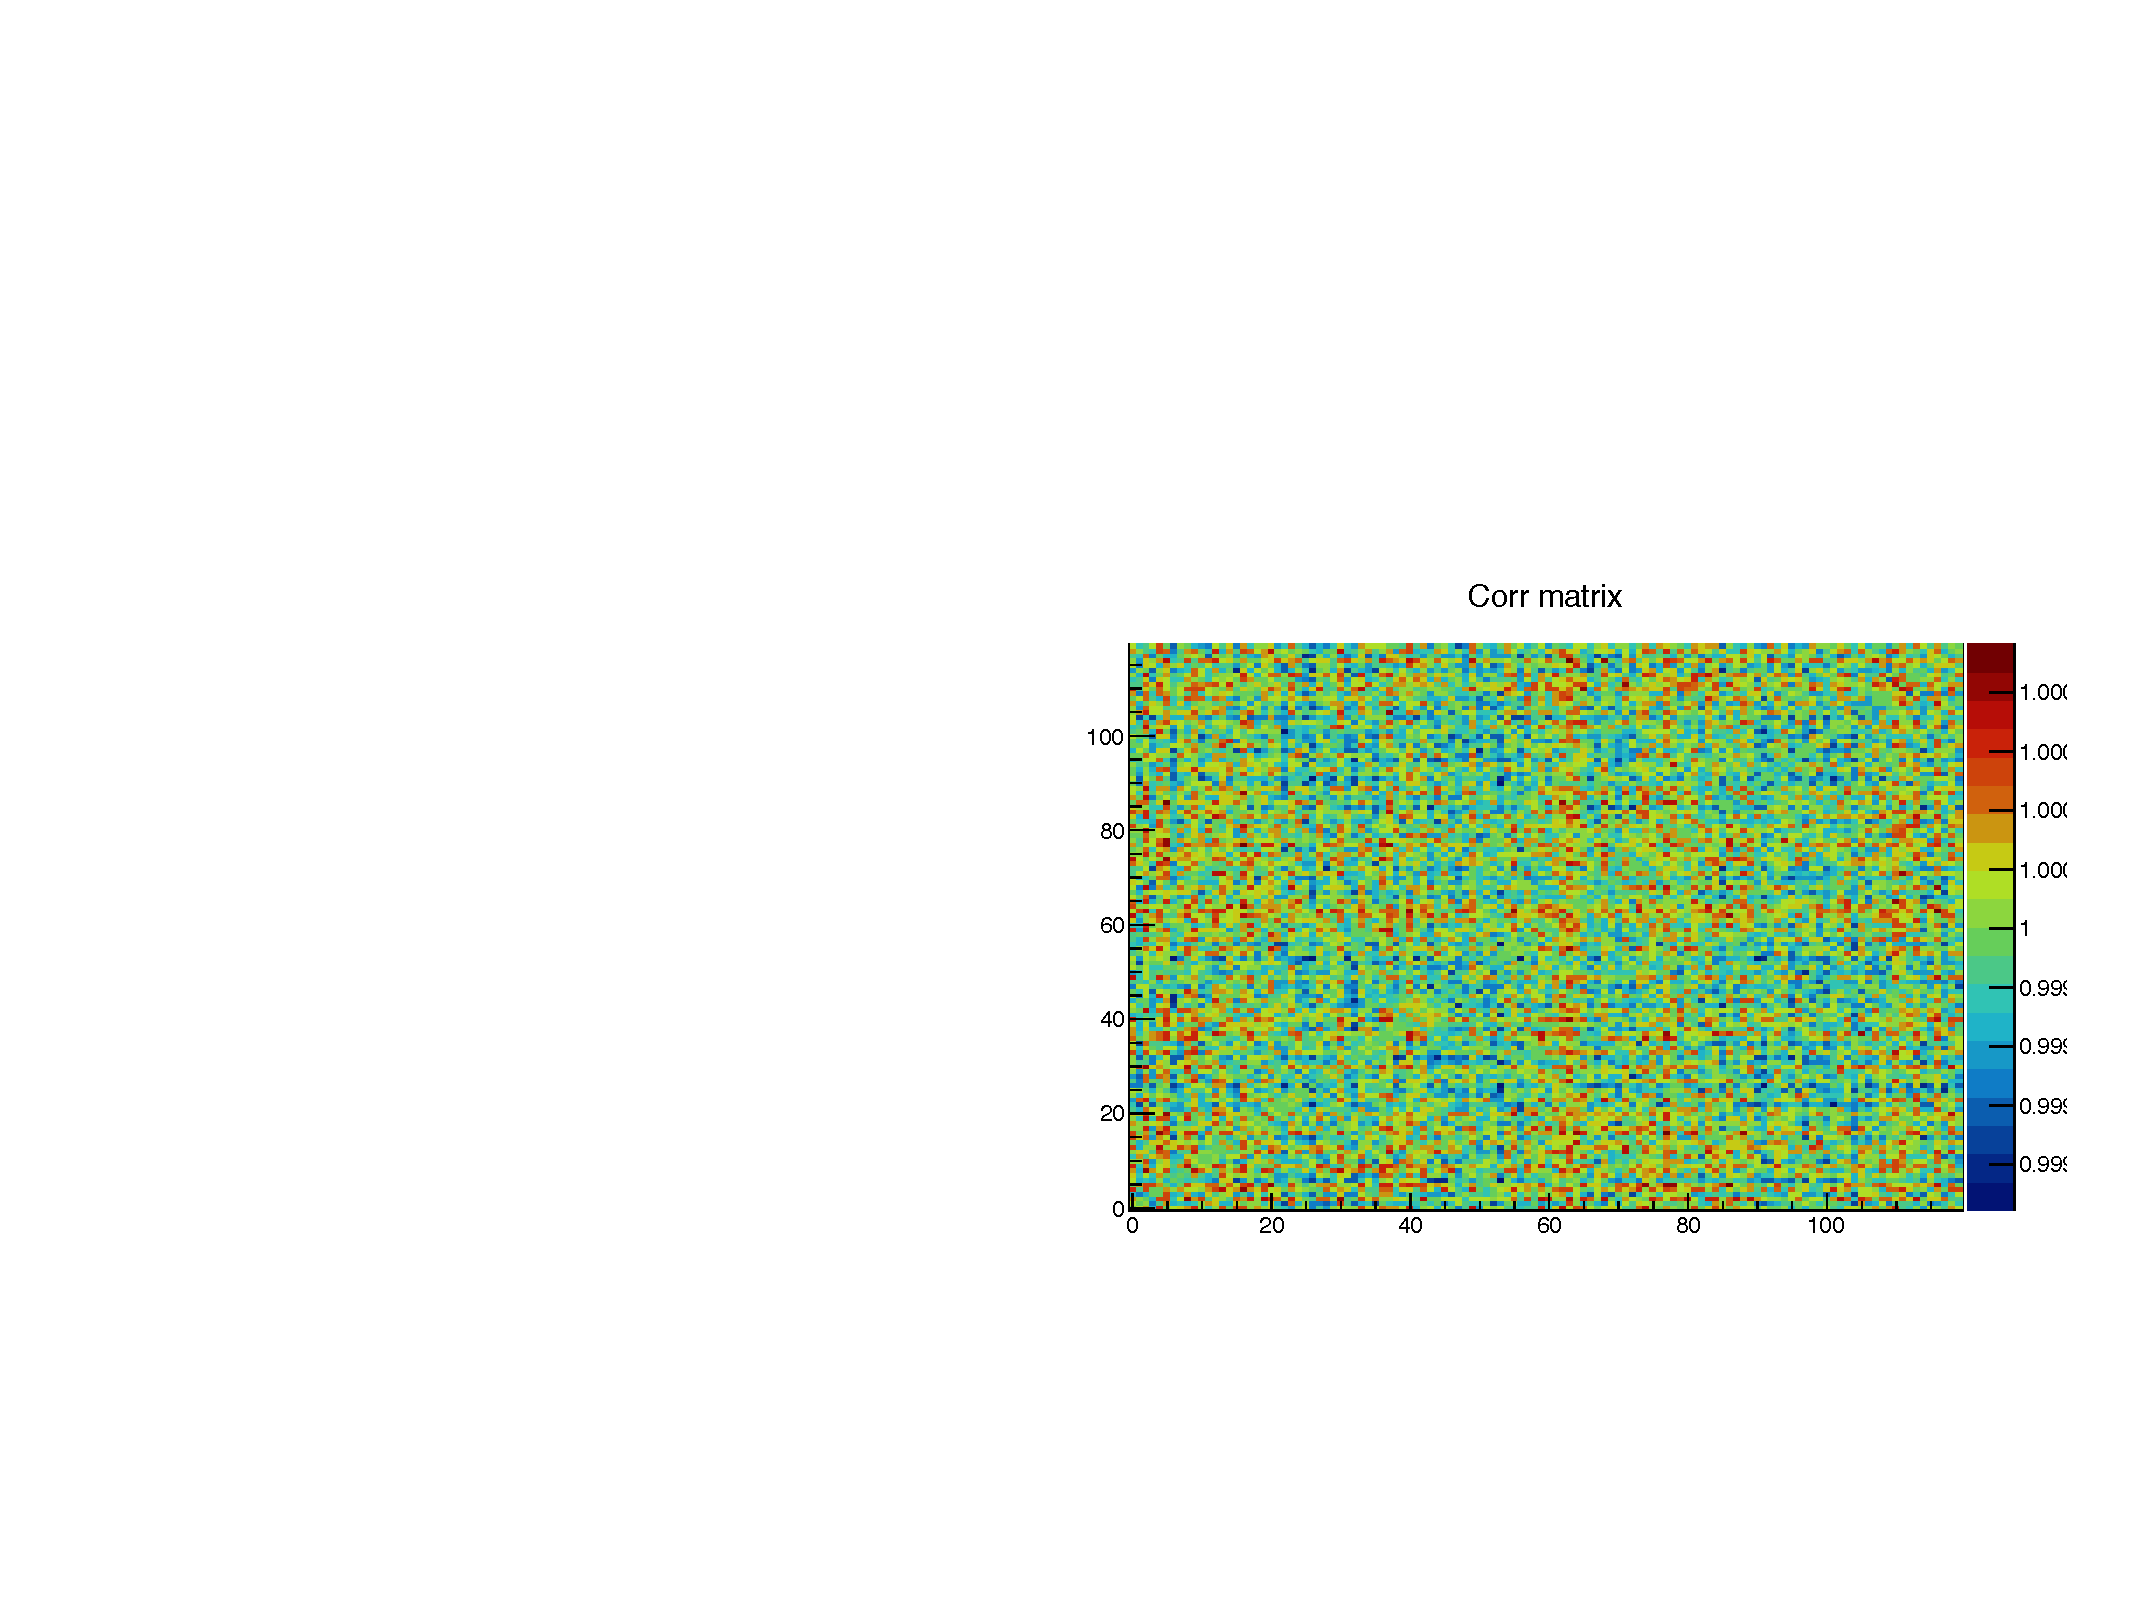
\includegraphics[width=0.49\linewidth]{plots/170109_Unal_mh_syst_corrALL.pdf}
  \hfill
  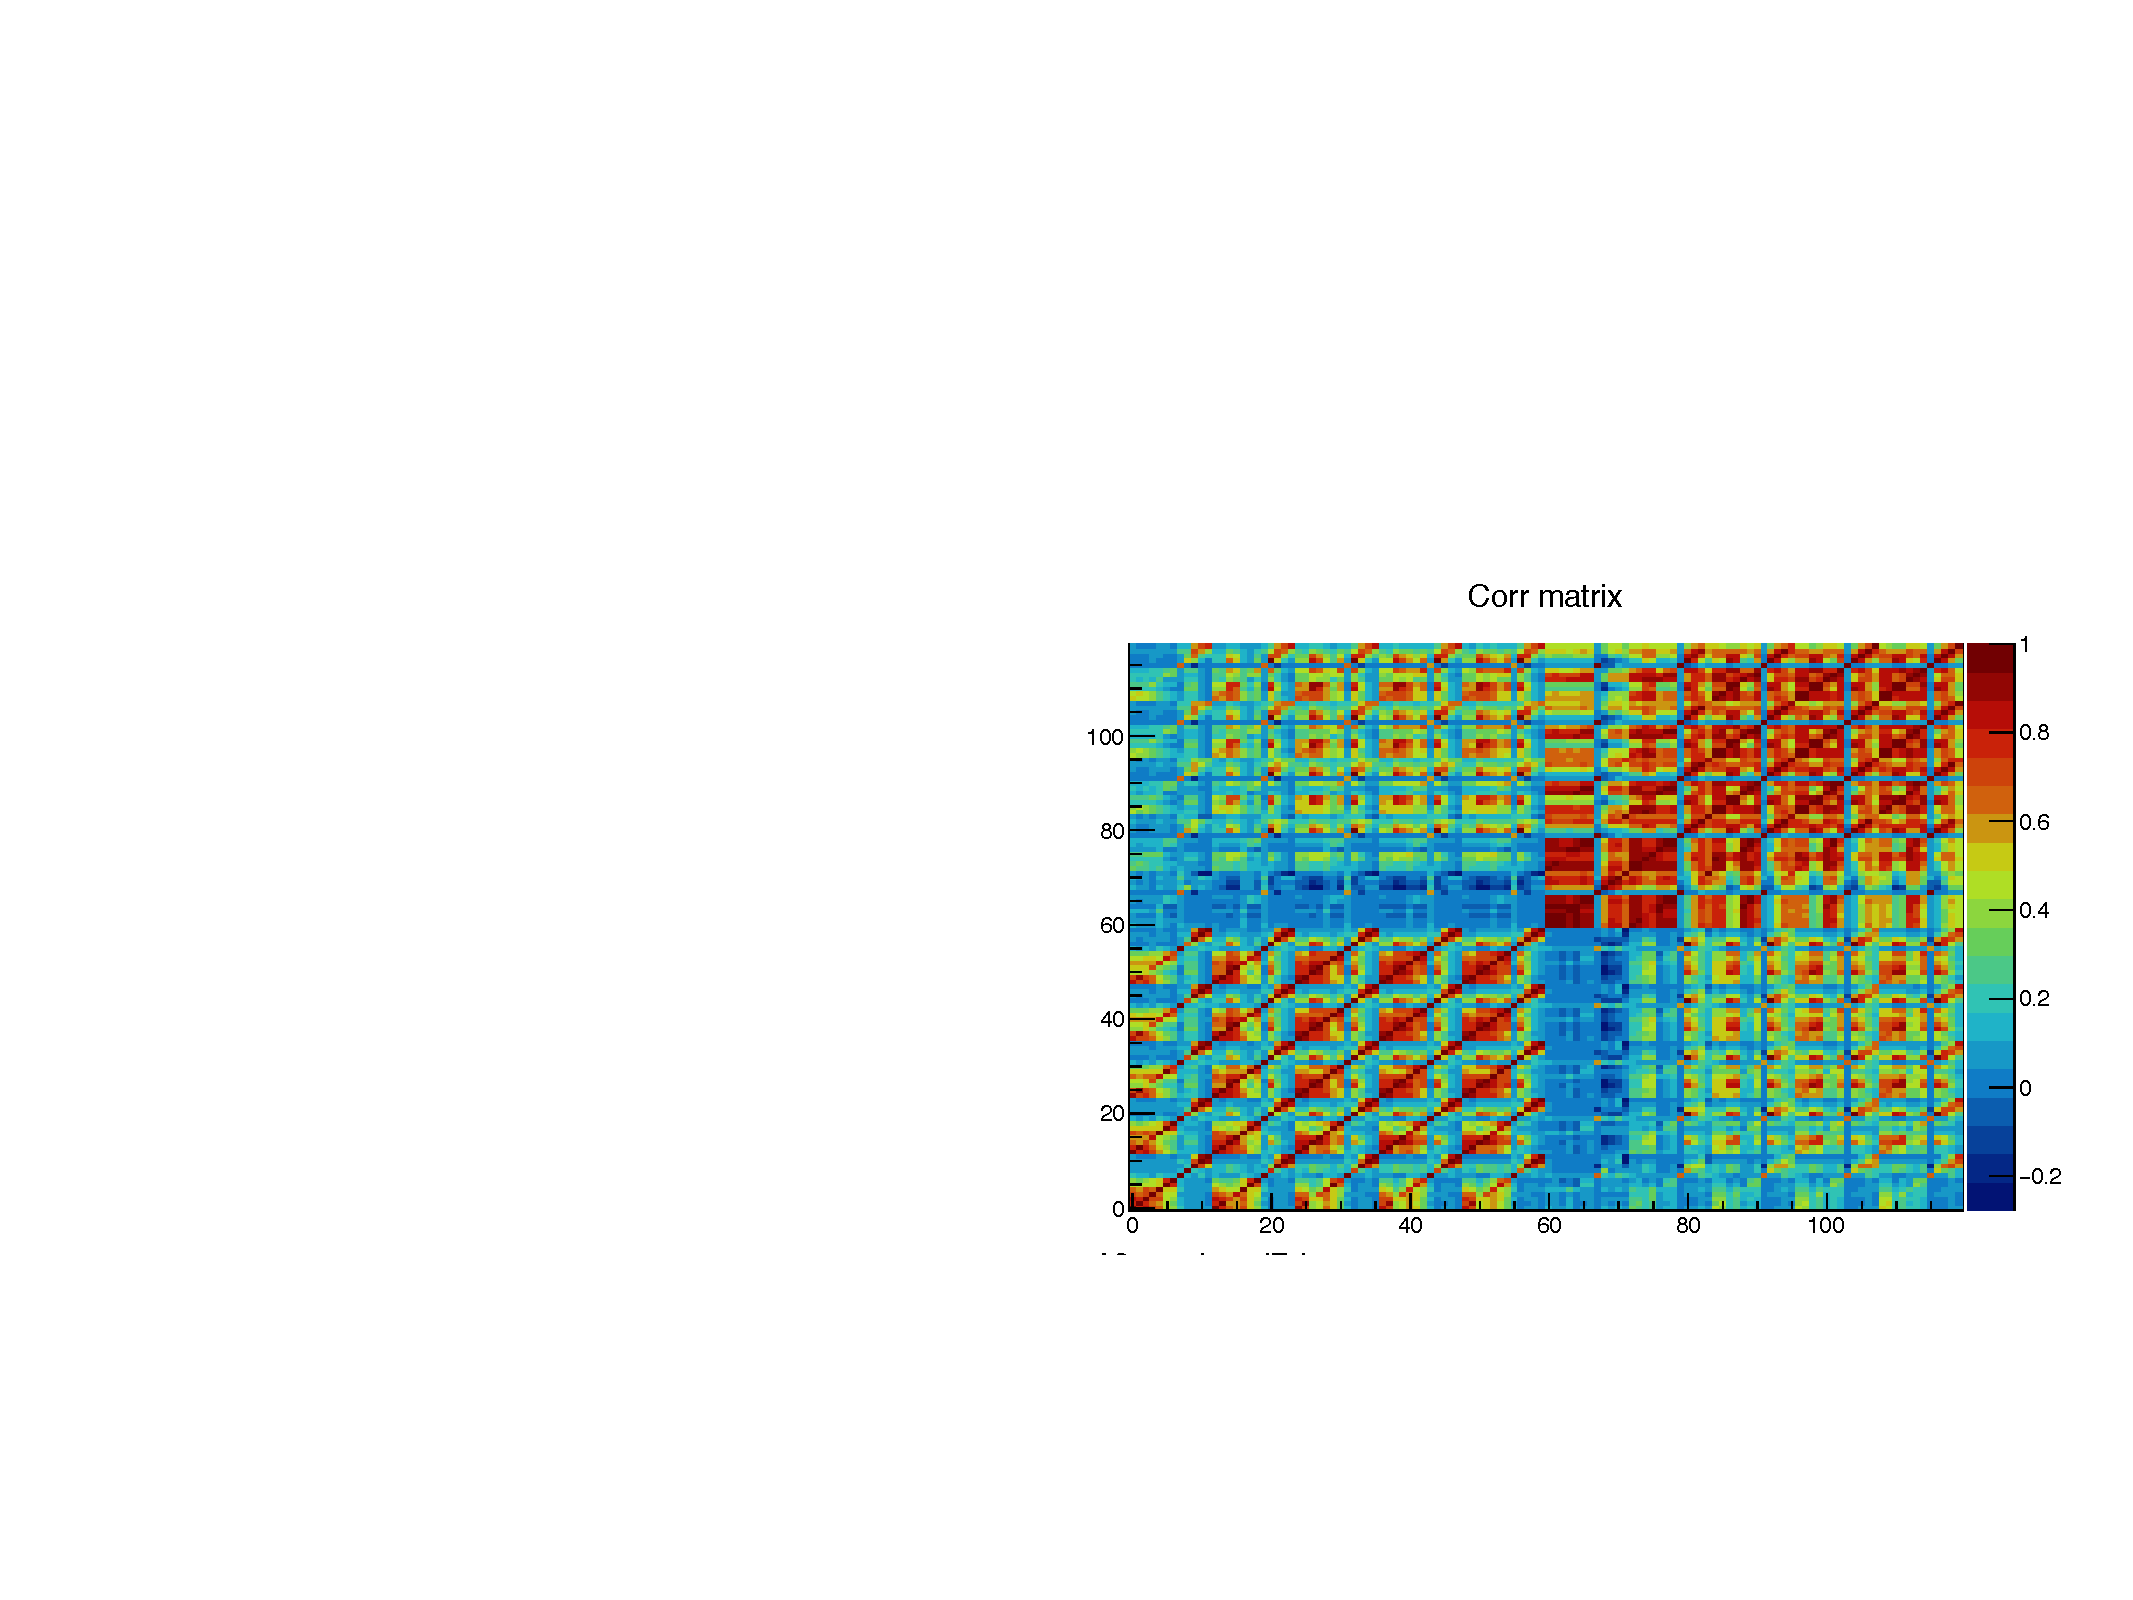
\includegraphics[width=0.49\linewidth]{plots/170109_Unal_mh_syst_corrFULL.pdf}

  
  \begin{minipage}{0.49\linewidth} $$\frac{\sigma_M}{M}=0.47\%$$\end{minipage}
  \hfill
  \begin{minipage}{0.49\linewidth}$$\frac{\sigma_M}{M}=0.26\%$$ \end{minipage}

  \vfill
  Cross-checks validate values obtained by mass fitting.
  \end{frame}
  %==================================================
  \begin{frame}{Category comparison}
    The previous inclusive results are compared to asimov with 13 categories.

    \begin{center}
      Total Scale Uncertainty :\\
      \begin{tabular}{l|rrr}
        \% & ALL & FULL & ratio\\
        \hline
        Mass fit & 0.46 & 0.27 & 41\\
        Formula & 0.47 & 0.26 & 45\\
        Asimov & 0.53 & 0.34 & 36\\
      \end{tabular}
    \end{center}

    Bad calibration categories have a higher contribution to the resolution.
  \end{frame}

  
  %==================================================
%% \begin{frame}{old}
%% \end{frame}
%% \begin{frame}{Method comparison}
%%   4 different fitting methods are compared : fitting in 3 different ranges and template method cross-check within $[122, 128]$GeV.
%%   Methods compared on h013 simplified model (2NP).
  
%%   \begin{minipage}{0.42\linewidth}
%%    % $$m_{\gamma\gamma}\in [105,160]$$
%%     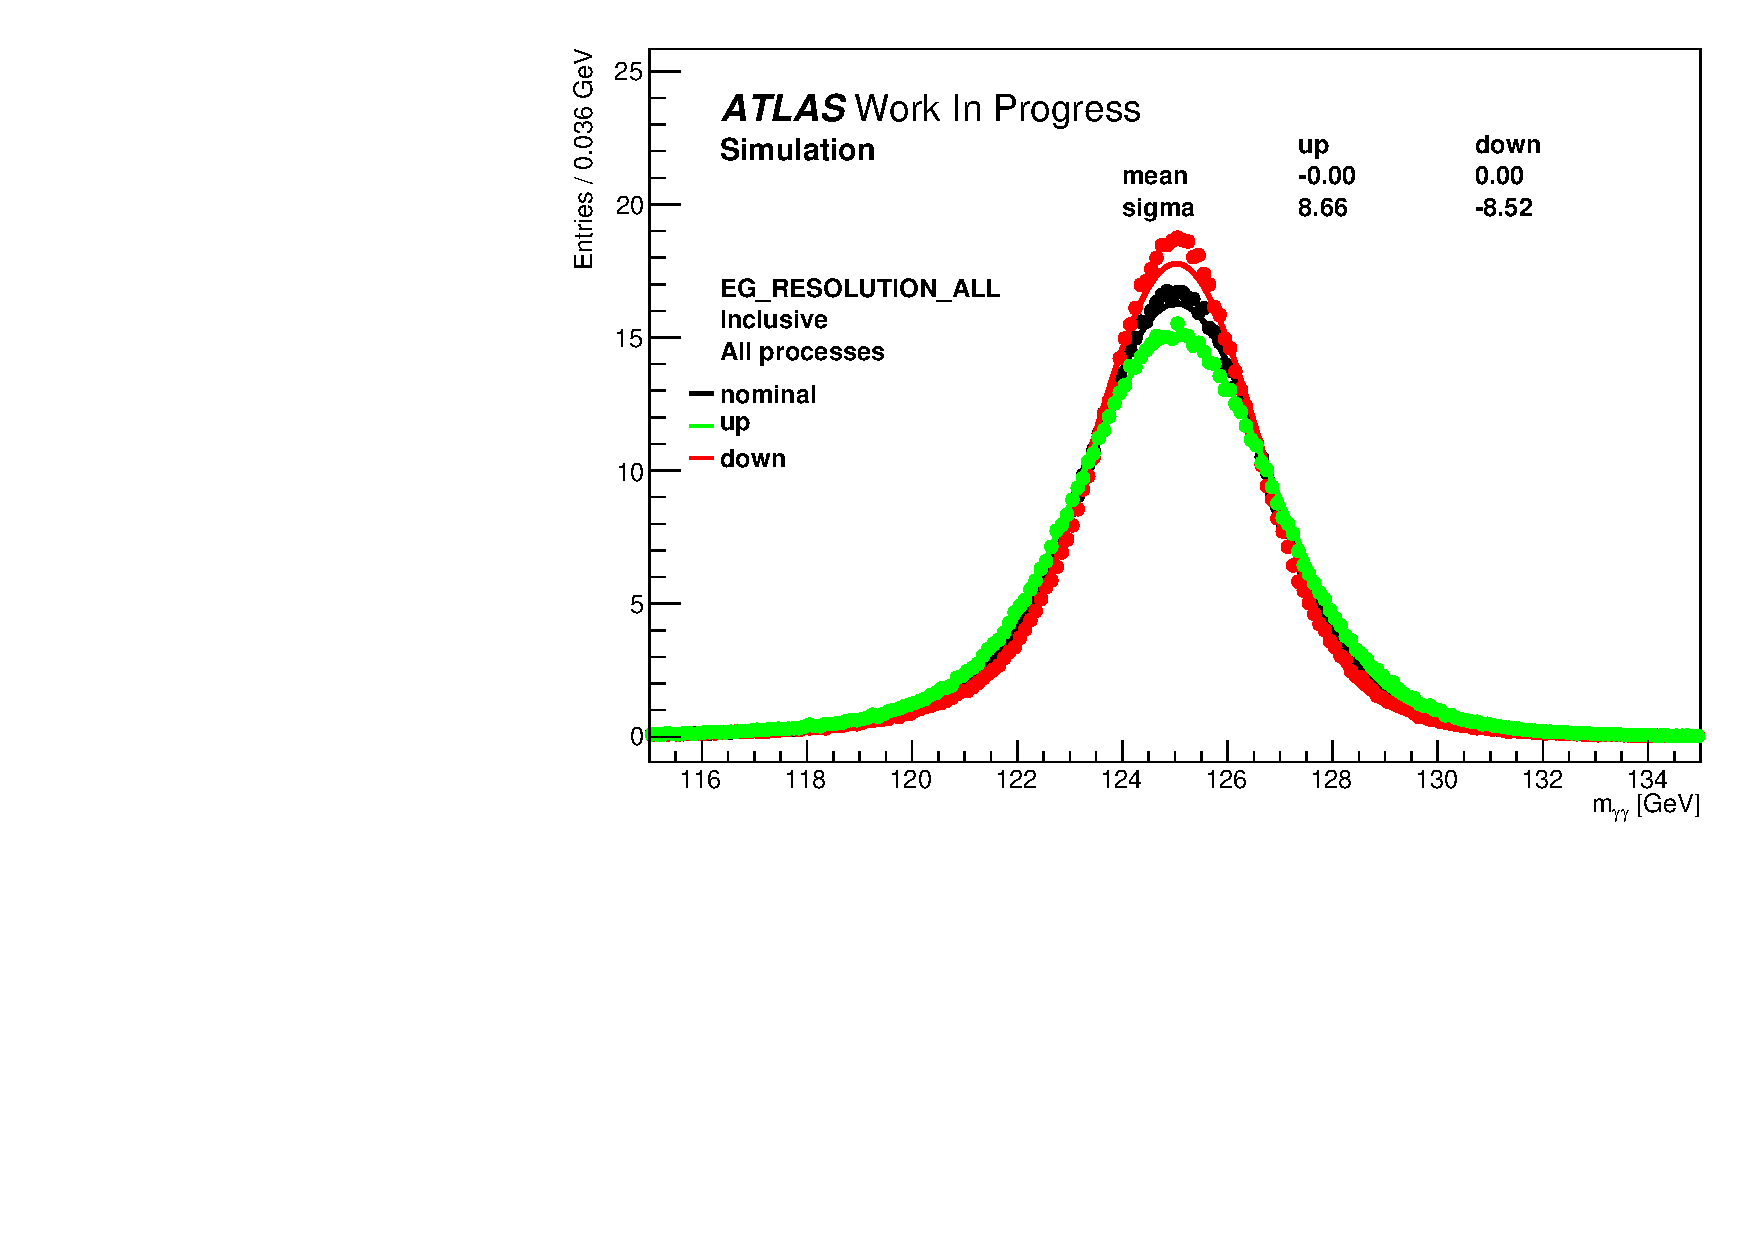
\includegraphics[width=\linewidth]{plots/h013_EG_RESOLUTION_ALL_0_105160.pdf}
%%   \end{minipage}
%%   \hfill
%%   \begin{minipage}{0.14\linewidth}
%%     $\leftarrow [105,160]$
%%     $\rightarrow [115,135]$
%%     \end{minipage}
%%   \hfill
%%   \begin{minipage}{0.42\linewidth}
%%     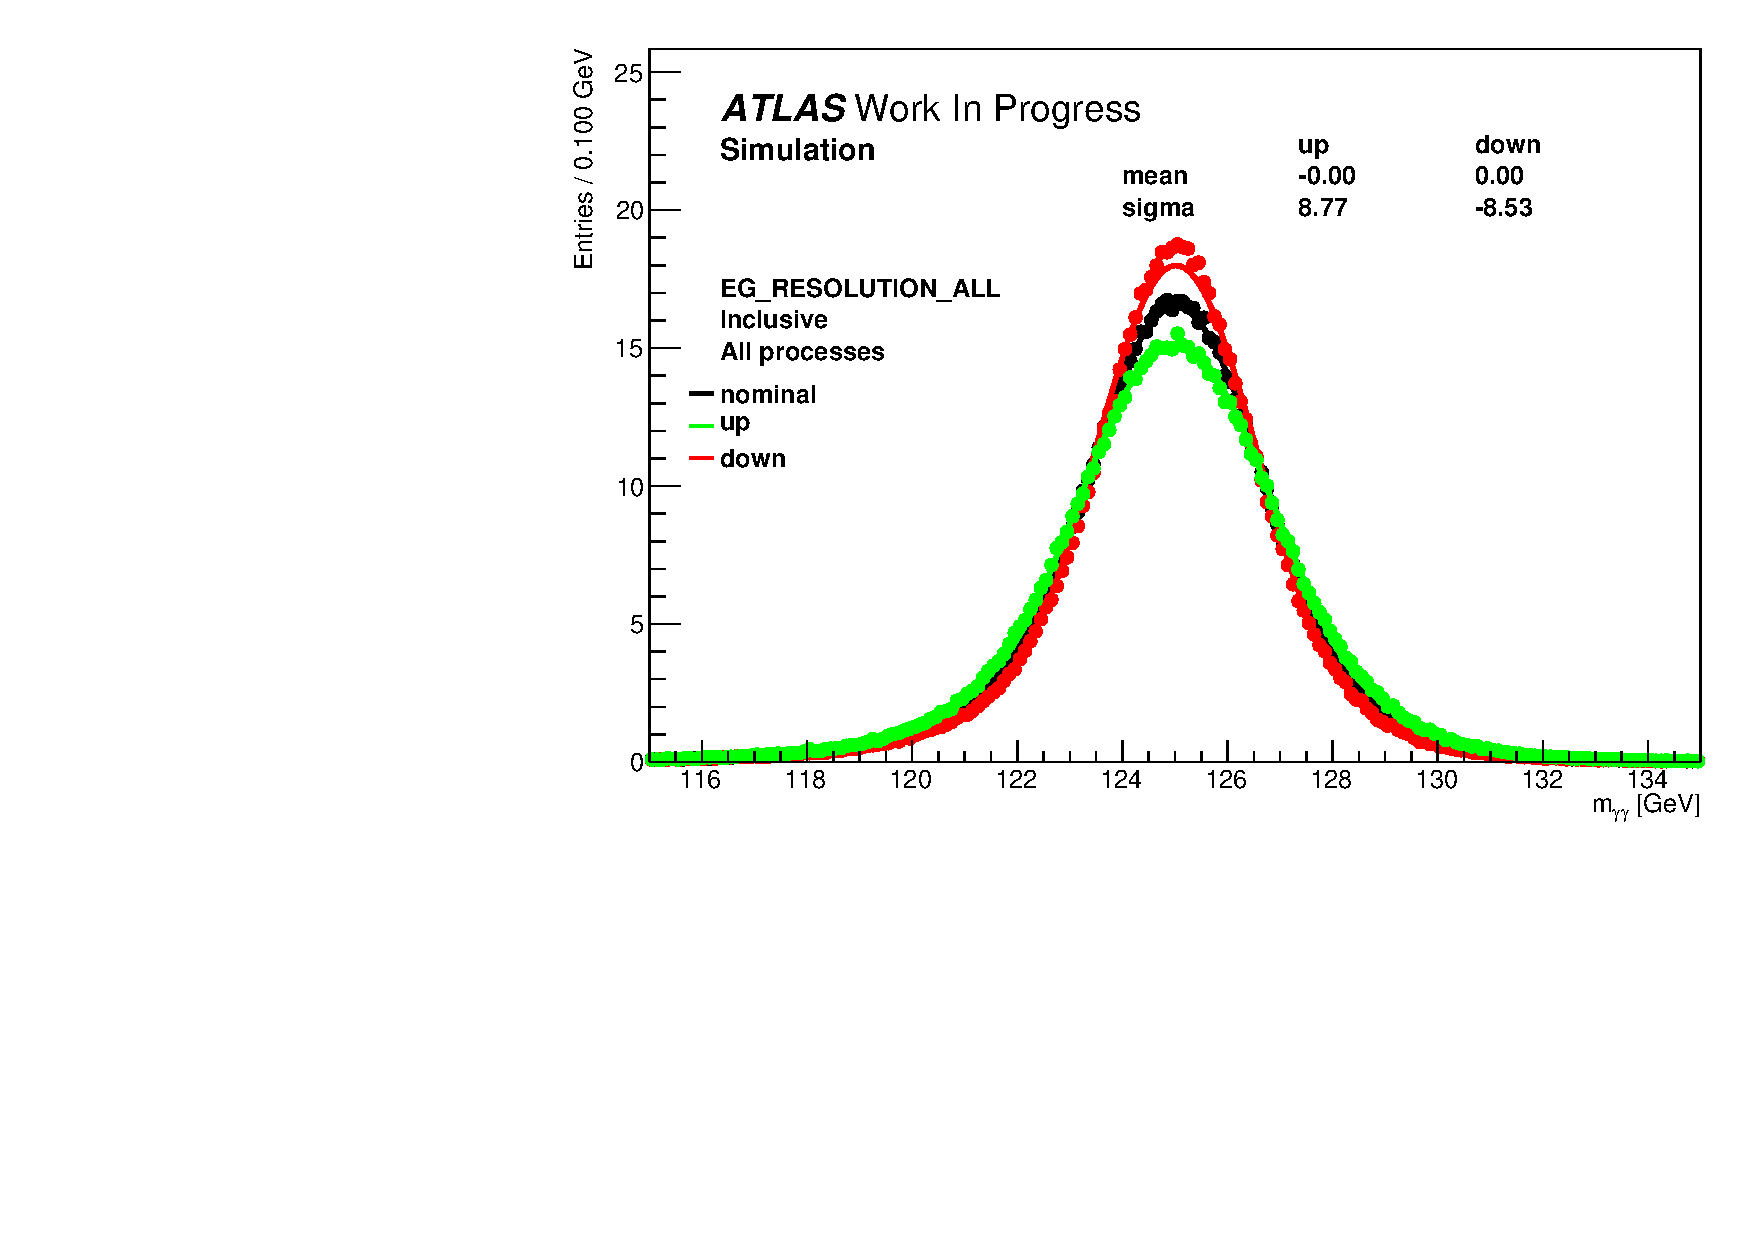
\includegraphics[width=\linewidth]{plots/h013_EG_RESOLUTION_ALL_0_115135.pdf}
%%   \end{minipage}
%%   \begin{minipage}{0.42\linewidth}
%%     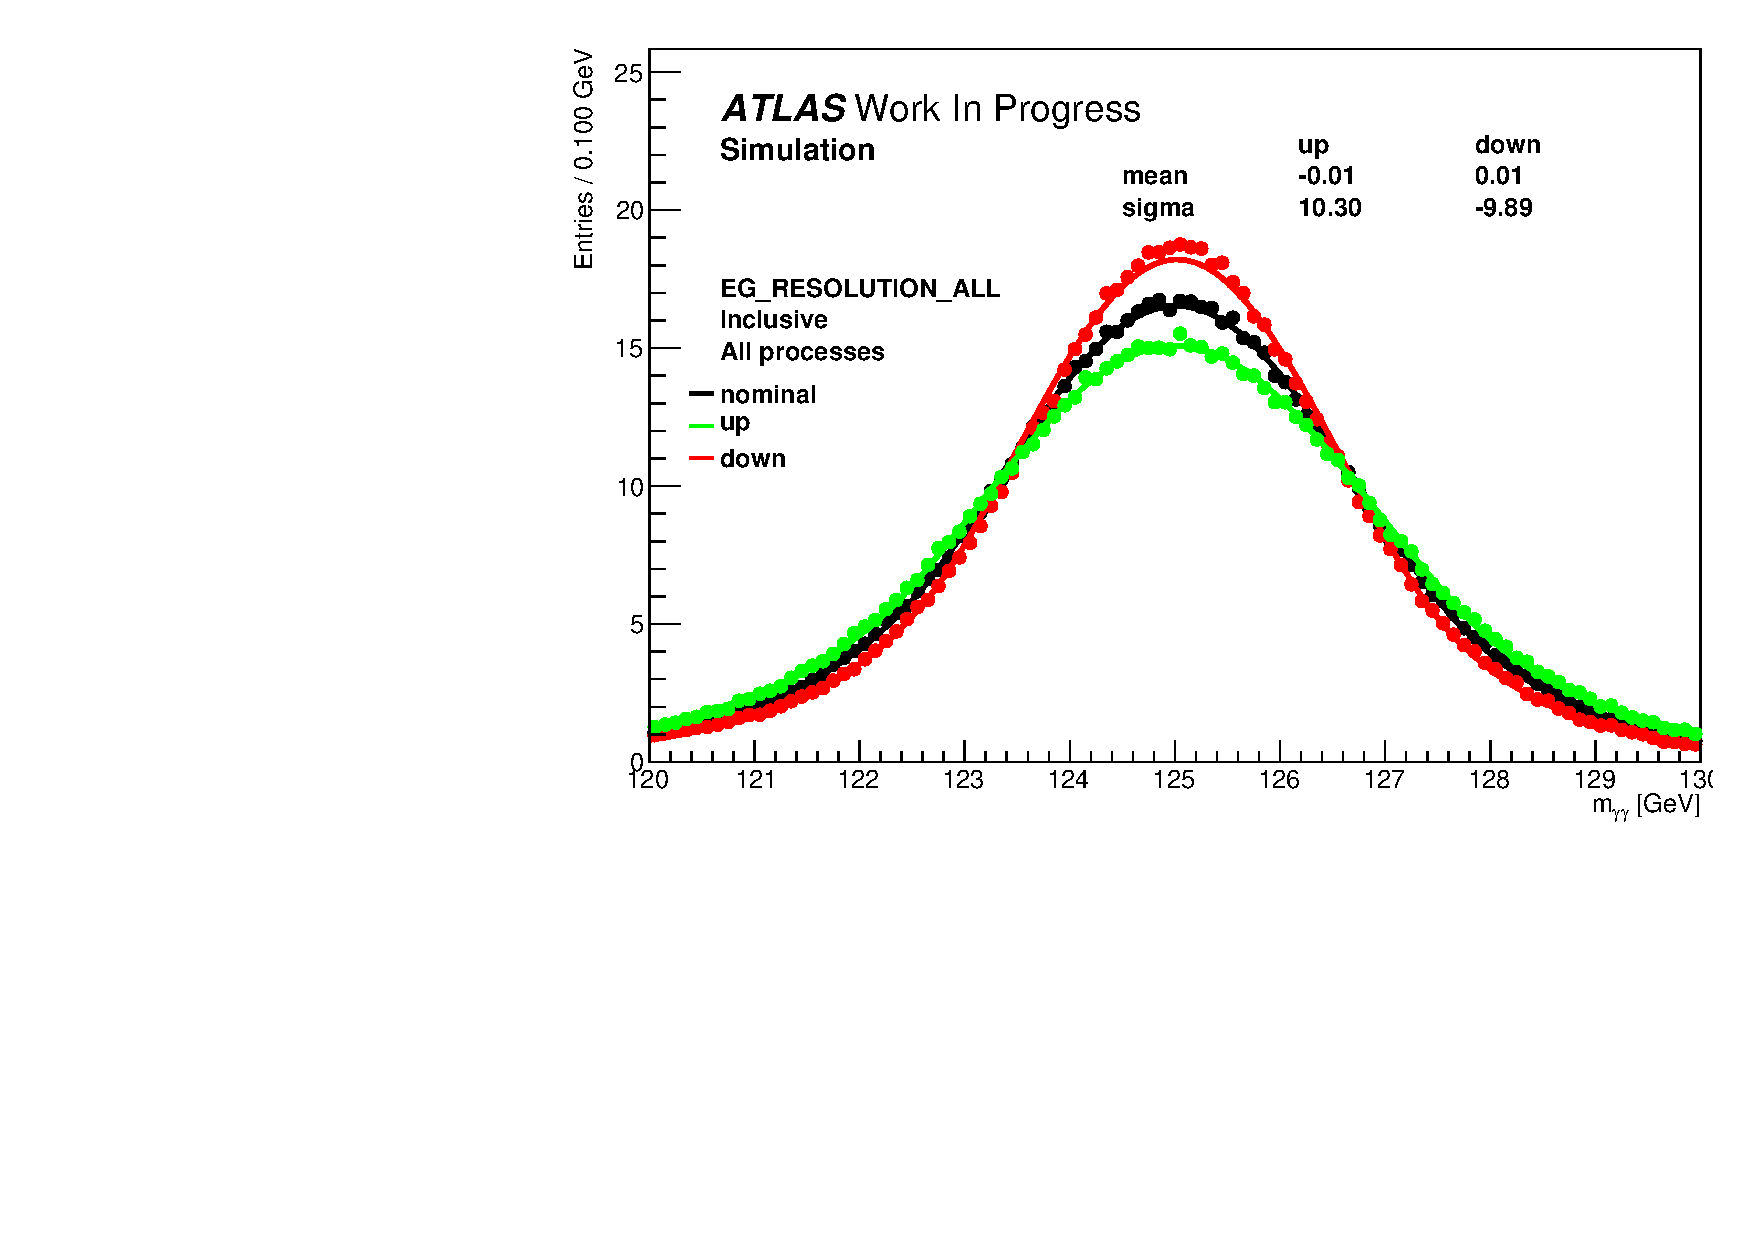
\includegraphics[width=\linewidth]{plots/h013_EG_RESOLUTION_ALL_0_120130.pdf}
%%   \end{minipage}
%%   \hfill
%%   \begin{minipage}{0.14\linewidth}
%%     $\leftarrow [120,130]$
%%     $\rightarrow [122,128]$
%%   \end{minipage}
%%     \hfill
%%   \begin{minipage}{0.42\linewidth}
%%     \centering
%%         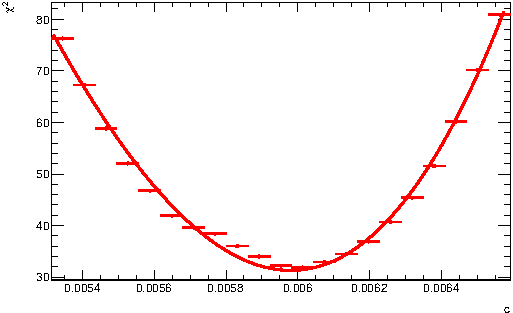
\includegraphics[width=0.5\linewidth]{plots/h013_EG_RESOLUTION_ALL__1up_0_scale.pdf}\\
%%         $c=(0.598\pm 0.009)\%$\\$\rightarrow \delta_{\sigma_H}=(8.82\pm0.25)\%$
%%   \end{minipage}
%% \end{frame}

%% %%=================================================================================
%% \begin{frame}{Calibration systematics model discrepancies}
%%   \begin{minipage}{0.49\linewidth}
%%     \begin{itemize}
%%     \item RESOLUTION\_ZSMEARING should be identical to RESOLUTION\_ALL.
%%     \item Distributions agree but not fits
%%     \item Will look into fit procedure.
%%     \end{itemize}
%%   \end{minipage}
%%   \hfill
%%   \begin{minipage}{0.49\linewidth}
%%     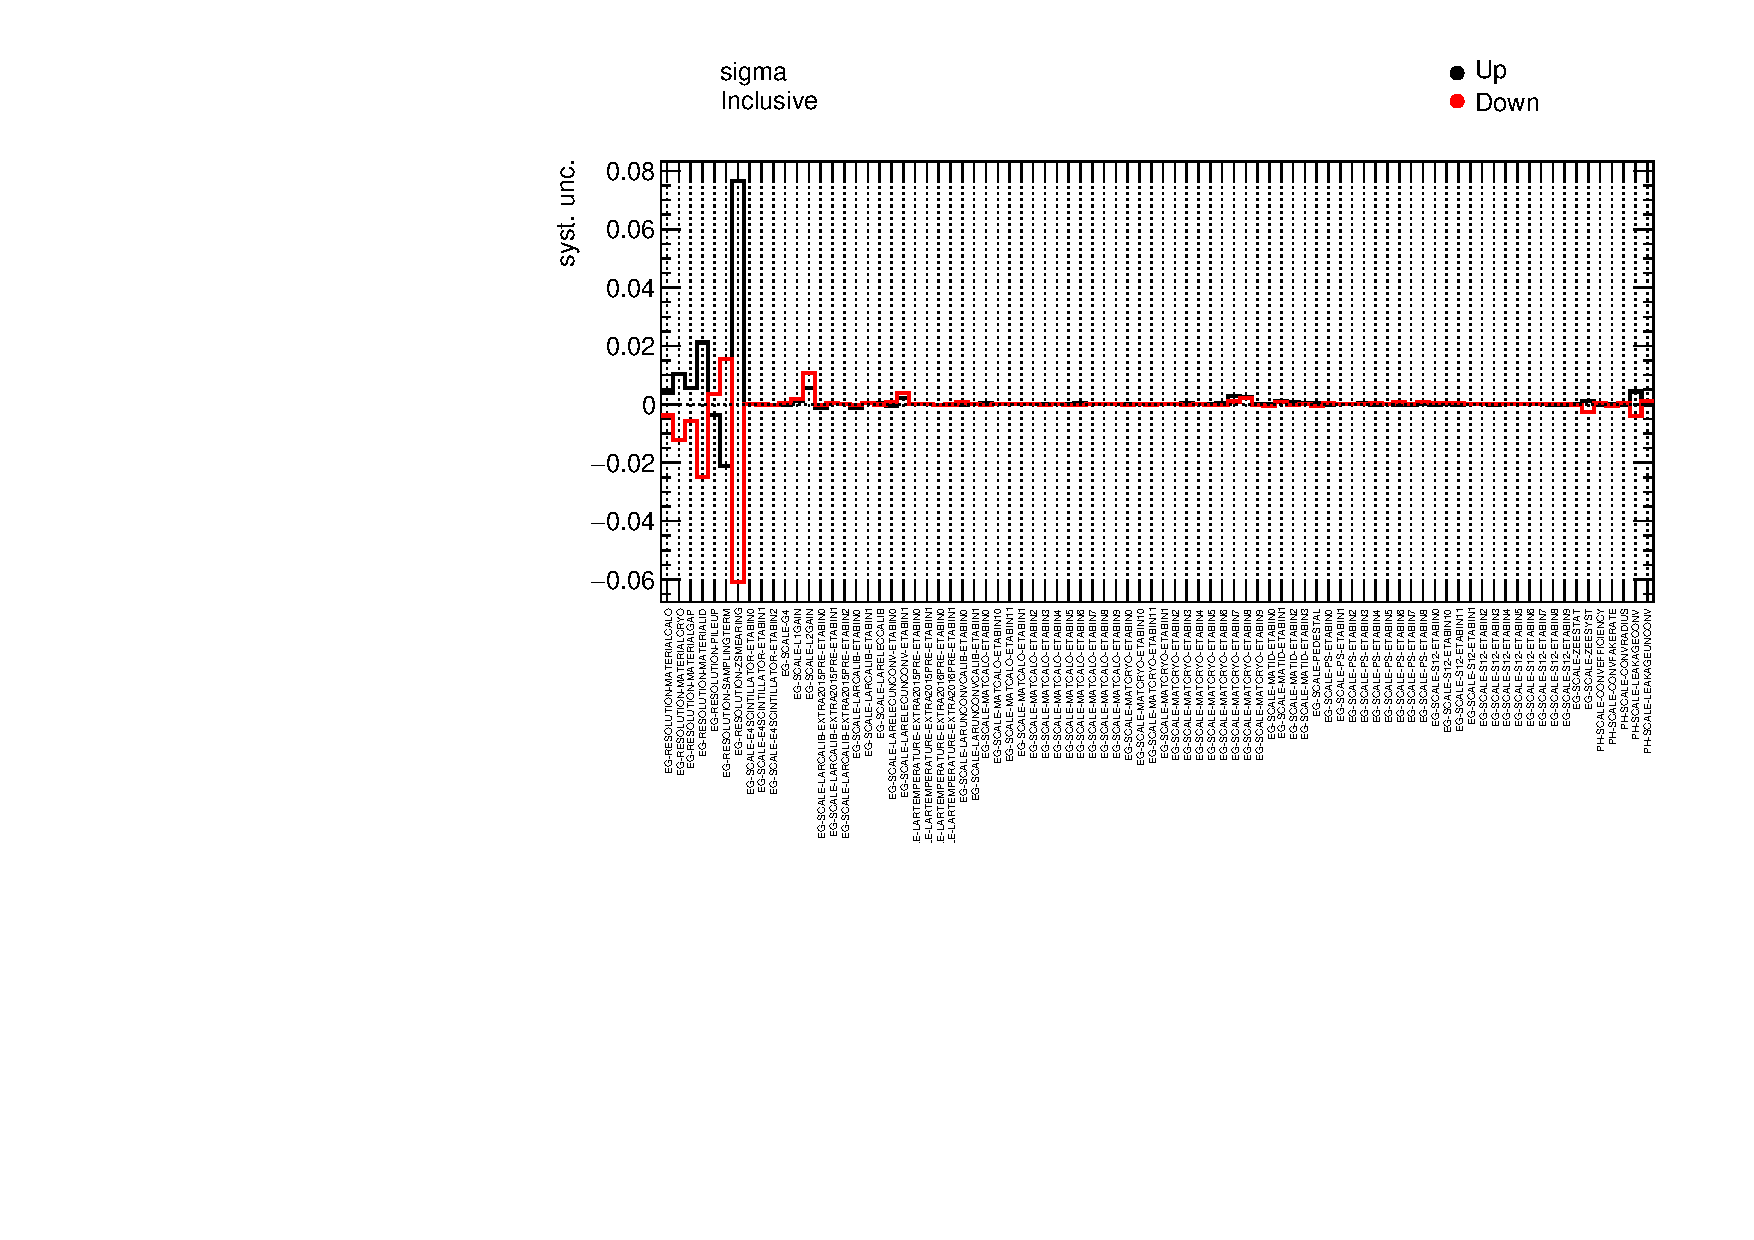
\includegraphics[width=\linewidth]{plots/allSyst_sigma_Inclusive_sigma.pdf}\\
%%   \end{minipage}
%%   \begin{minipage}{0.49\linewidth}
%%     \begin{center}
%%       Total Inclusive Uncertainty :
%%       \begin{tabular}{l|rr}
%%         \% & Scale & Resolution \\
%%         \hline
%%         Full & 0.26 & 7.03 \\
%%         Reduced & 0.44 & 11.11 \\
%%       \end{tabular}
%%     \end{center}
%%   \end{minipage}
%%   \hfill
%%   \begin{minipage}{0.49\linewidth}
%%     \includegraphics[width=\linewidth]{/home/goudet/Bureau/LAL/Zim/Hgam/PhotonSystematic/161220_CompareModels_m_yy.pdf}
%%   \end{minipage}
%% \end{frame}

%% %%==============================================================
%% \begin{frame}{Method impact on values}
%%   \begin{center}
%%     FULL and ALL models are compared with a fit within $[115,135]$.
%%     \adjustbox{width=\linewidth}{
%%     \begin{tabular}{rrrrrrrr}
%%       NP&cat&mean&sigma&alphaHi&alphaLow&nHi&nLow\\
%%       \hline
%%       nominal ALL  &0&125.014&1.7421&1.48071&1.34134&19.9948&7.91861\\
%%       nominal FULL&0&124.998&1.77225&1.47488&1.37898&19.9071&7.56628\\
%%       \hline
%%       Difference (\%) & & & 1.7& 2.8& & 4.4\\
%%       \hline
%%       EG\_RESOLUTION\_ALL\_\_1up&0&125.009&1.89485&1.48071&1.34134&19.9948&7.91861\\
%%       EG\_RESOLUTION\_ZSMEARING\_\_1up&0&124.993&1.90455&1.47488&1.37898&19.9071&7.56628\\
%%       \hline
%%       Difference (\%) & & & 0.5& & & \\
%%       \hline
%%     \end{tabular}
%%     }
%%         \includegraphics[width=0.5\linewidth]{/home/goudet/Bureau/LAL/Zim/Hgam/PhotonSystematic/161220_CompareModels_m_yy.pdf}
%%     \end{center}
%% \end{frame}


%% %%==============================================================
%% \begin{frame}{Comparison with ZSMEARING}
%%   \begin{minipage}{0.49\linewidth}
%%     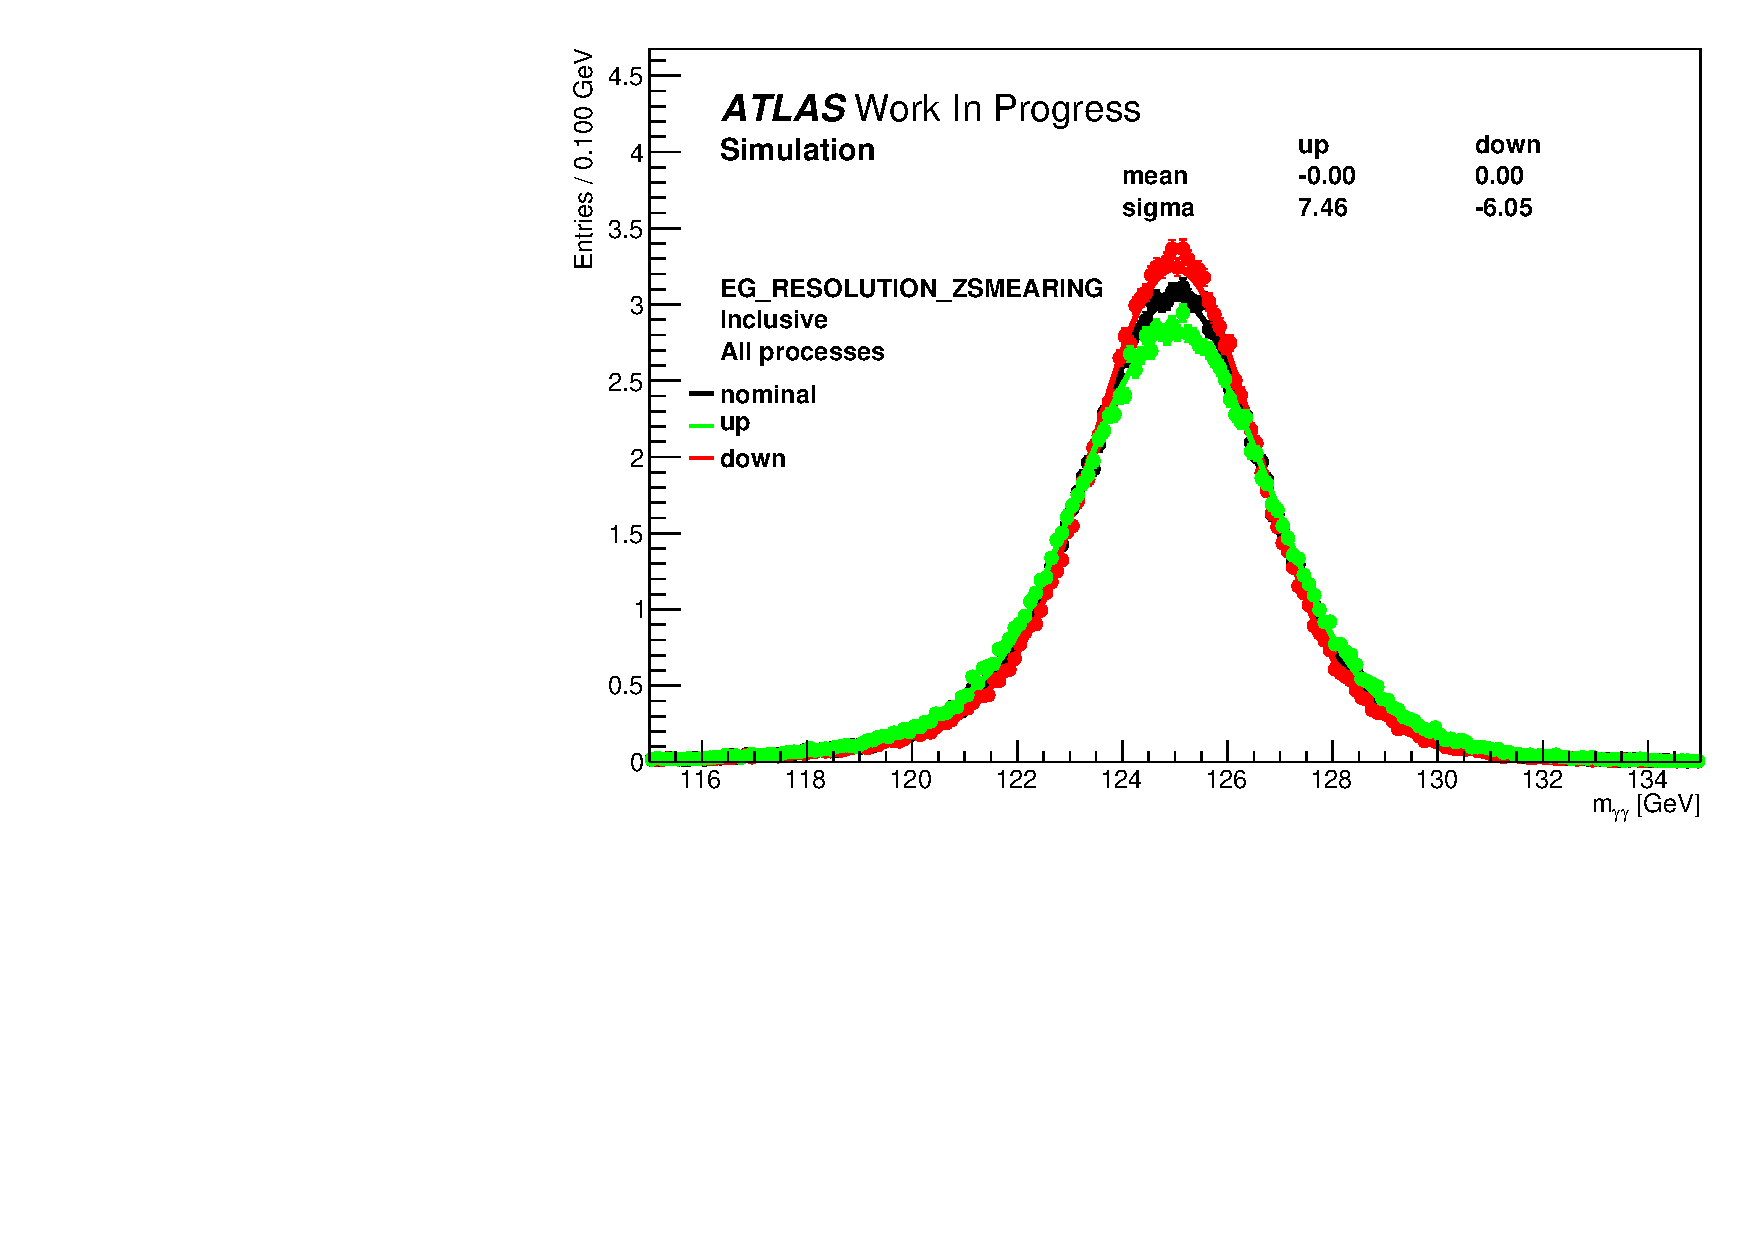
\includegraphics[width=\linewidth]{plots/h013_EG_RESOLUTION_ZSMEARING_0_125135.pdf}
%%     $$\sigma_H = (1.77 \pm 0.37)\%$$
%%   \end{minipage}
%%   \hfill
%%   \begin{minipage}{0.49\linewidth}
%%         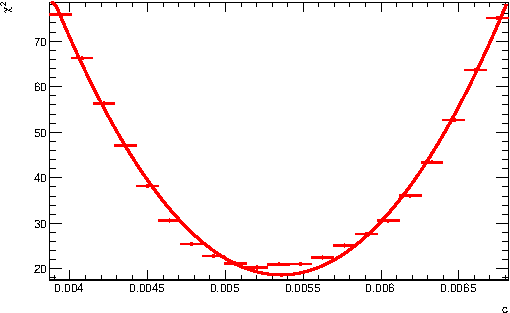
\includegraphics[width=\linewidth]{plots/h013_EG_RESOLUTION_ZSMEARING__1up_0_scale.pdf}
%%     $$c=(0.536 \pm 0.019) \%$$$$\rightarrow \delta_{\sigma_H} = (6.90 \pm 0.47)\%$$
%%   \end{minipage}
%%   \begin{center}
%%     \begin{tabular}{|l|r|r|}
%%       \hline
%%     $(\pm 0.5)$\% &Fit $[115, 135]$& Template $[122, 128]$\\
%%     \hline
%%     RESOLUTION\_ALL & 8.77 & 8.82\\
%%     RESOLUTION\_ZSMEARING & 7.46 &6.9\\
%%     \hline
%%     \end{tabular}

%% \end{center}
%% \end{frame}
%% %%==============================================================
%% \begin{frame}{Simplified model}
%%   The simplified model sum in quadrature respectively all systematic sources into respectively a single nuisance parameter for scale and resolution.
%%   The fit between $[115,135]$ is used as closest to the signal model tool default behaviour.

%%   \begin{minipage}{0.49\linewidth}
%%     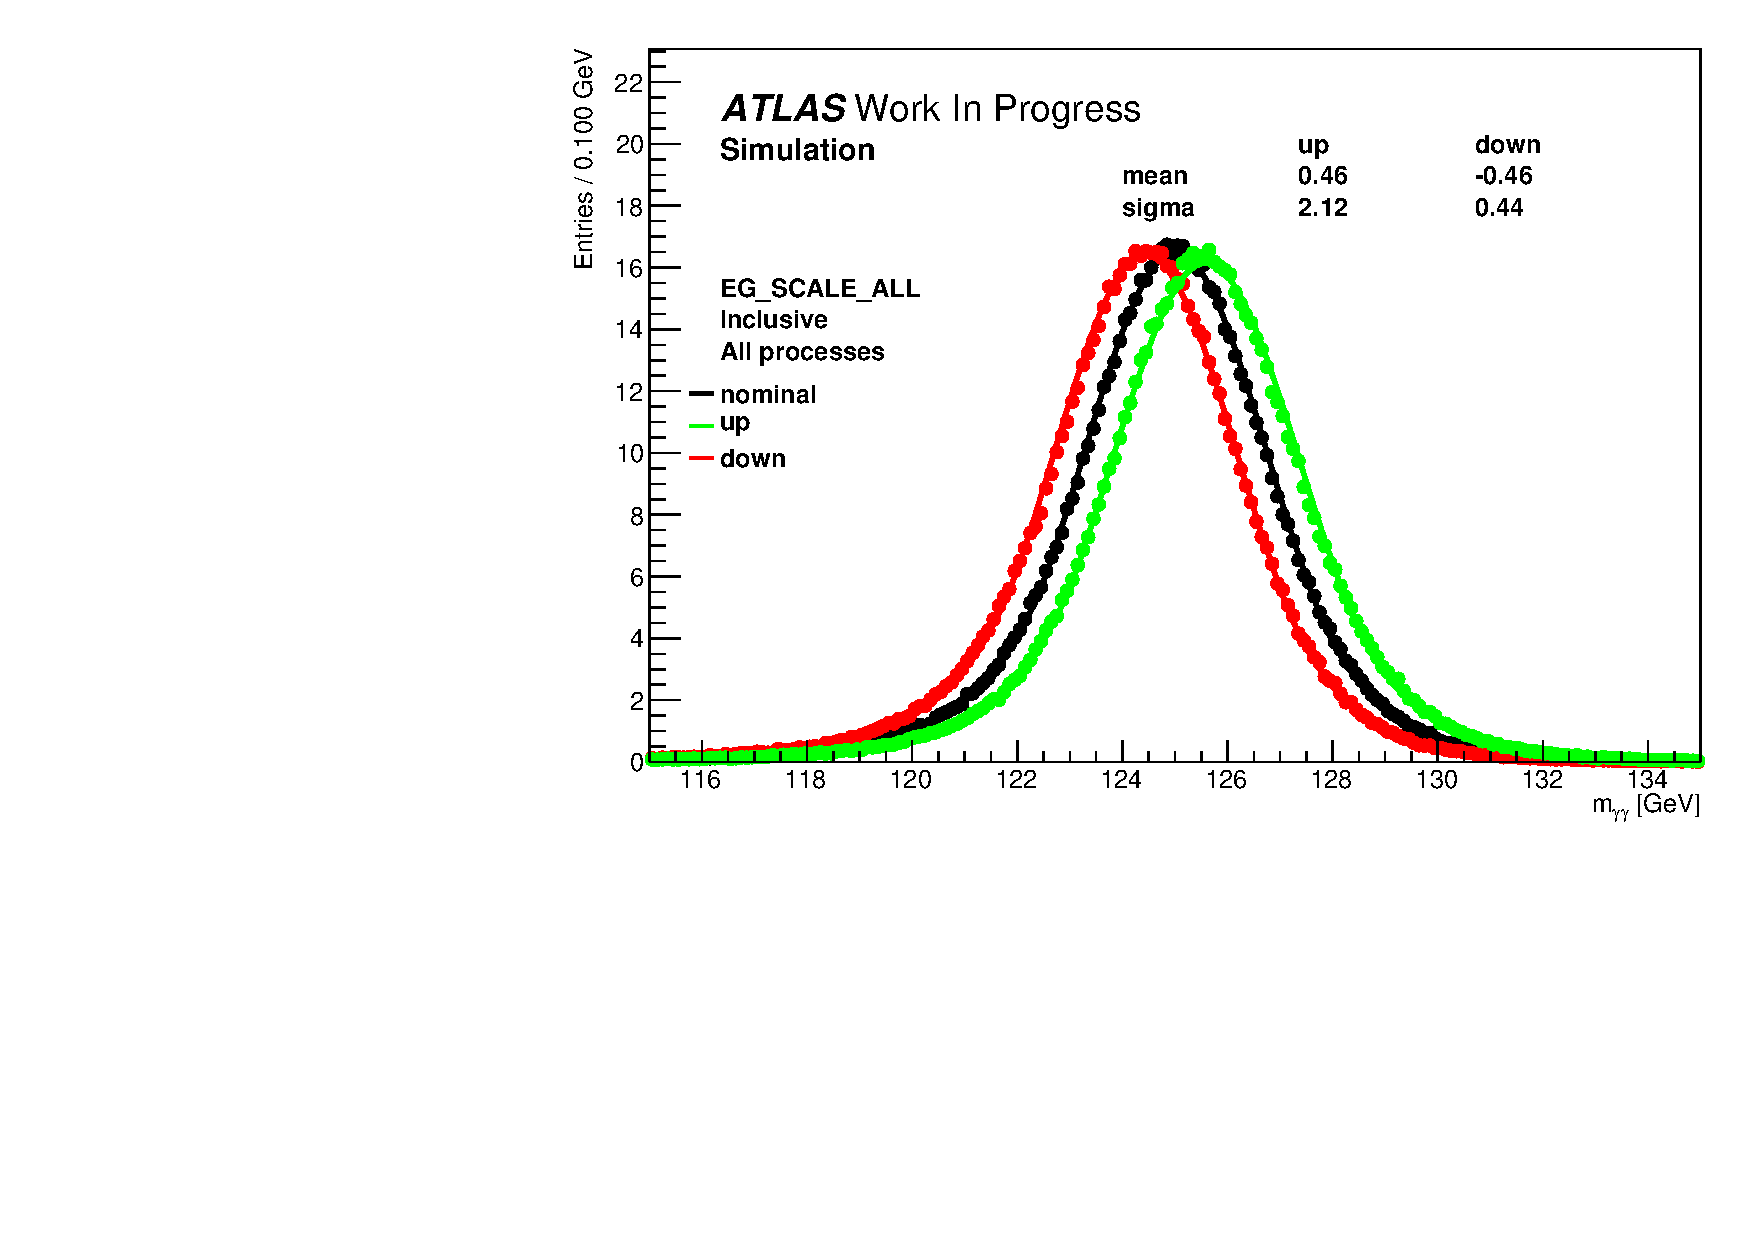
\includegraphics[width=\linewidth]{plots/h013_EG_SCALE_ALL_0_115135.pdf}
%%   \end{minipage}
%%   \hfill
%%   \begin{minipage}{0.49\linewidth}
%%     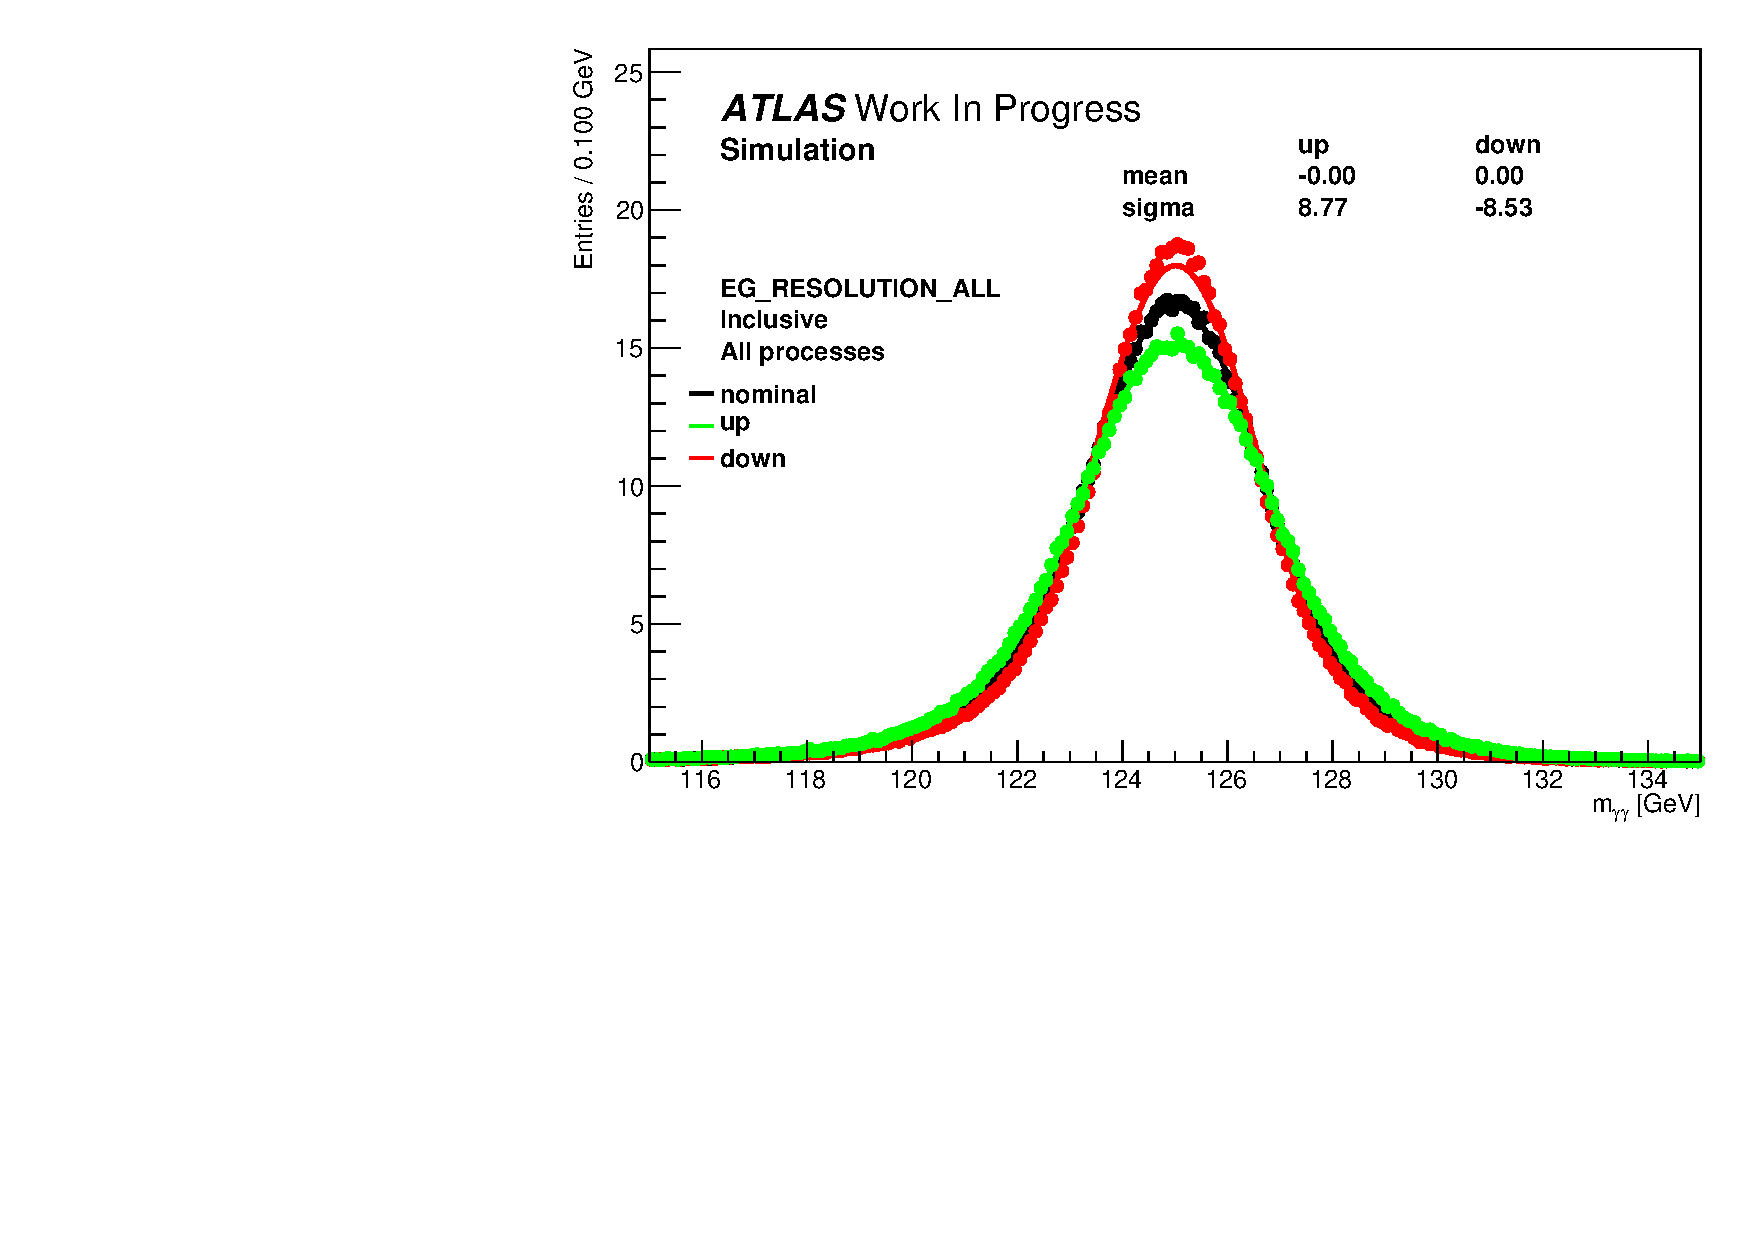
\includegraphics[width=\linewidth]{plots/h013_EG_RESOLUTION_ALL_0_115135.pdf}
%%   \end{minipage}  
%% \end{frame}

%% %%=================================================================================
%% \begin{frame}{Model FULL\_v1 : mass uncertainty}
%%   The full model (83 NP) is used instead of simplified 3NP model.
%%   \vfill
%%   \includegraphics[width=0.9\linewidth]{/home/goudet/Documents/LAL/Zim/Hgam/PhotonSystematic/161220_h013_mean_Full_mean.pdf}
  
%% \end{frame}
%% %%=============================
%% \begin{frame}{Model FULL\_v1 : resolution uncertainty}
%%   The full model (83 NP) is used instead of simplified 3NP model.
%%   \vfill
%%   \includegraphics[width=0.9\linewidth]{/home/goudet/Documents/LAL/Zim/Hgam/PhotonSystematic/161220_h013_sigma_Full_sigma.pdf}
%% \end{frame}
  \begin{frame}{Conclusion}
    \begin{itemize}
    \item Differences in mass uncertainty between correlation models understood as theory expected.
    \end{itemize}
    \vfill
    Ongoing :
    \begin{itemize}
    \item Resolution difference between ALL and FULL using h014.
    \item Asymmetry in resolution 
    \end{itemize}
  \end{frame}
%% ###################################################################################
%%###################################################################################
%%###################################################################################
\begin{frame}
\maketitle
\end{frame}
\appendix
%%=================================================================================
\begin{frame}{Systematics in statistical framework}
  Changing an energy correction factor (by systematic fluctuation) affects several parameters.
  For current results, it is assumed that {\bf only the parameter $X$ targetted by the systematic (POI) is affected} (hence fixing the others).

  Only the parametrization of $X$ will contain the measured uncertainty $\delta_X$ :
  $$X\rightarrow X(1+\delta_X\theta)$$
  with $\theta$ a gaussian constrained free parameter.
  \vfill
  \textcolor{red}{In the framework, the pulling of the nuisance parameters only affects the main parameter of the systematic}
\end{frame}

%%=================================================================================
\begin{frame}{Typical plot}
  \begin{minipage}{0.49\linewidth}
    \includegraphics[width=\linewidth]{plots/Backup/h013_ICHEP_PhotonSyst_EG_SCALE_ALL_mean.pdf}\\
  \end{minipage}
  \begin{minipage}{0.49\linewidth}
    For a given fitted variable (here mean) :
    \begin{itemize}
    \item Full line : $\frac{\mu_{up}-\mu_{nominal}}{\mu_{nominal}}$
    \item Dashed line : $-\frac{\mu_{down}-\mu_{nominal}}{\mu_{nominal}}$
 
    \end{itemize}
  \end{minipage}

  Both lines should be superimposed in case of symmetric systematics.
  \end{frame}
%%=================================================%%=================================================================================
\begin{frame}{Scale impact on width}
  \begin{minipage}{0.49\linewidth}\includegraphics[width=\linewidth]{/home/goudet/Documents/LAL/Zim/Hgam/PhotonSystematic/160826_SpreadGauss.pdf}\end{minipage}
  \hfill
  \begin{minipage}{0.49\linewidth}
    1M random numbers generated on a Gaussian$(\mu=125, \sigma=1)$.
    \begin{itemize}
    \item Initial numbers distribution.
    \item \textcolor{red}{Half events multiplied by $1.002$.}
    \item \textcolor{blue}{Remaining  events multiplied by $1.005$.}
    \item \textcolor{magenta}{Combined distribution of \textcolor{red}{red} and \textcolor{blue}{blue}.}
    \end{itemize}
  \end{minipage}
  \vfill
  Mean (m) and RMS (s) of a fitted gaussians are given in the legend.
  Interpretationof the curve in the next slides.
\end{frame}

%%=================================================================================
\begin{frame}{Uncertainty reduction}
  \begin{minipage}{0.49\linewidth}\includegraphics[width=\linewidth]{/home/goudet/Documents/LAL/Zim/Hgam/PhotonSystematic/161124_SpreadGauss_syst.pdf}\end{minipage}
  \hfill
  \begin{minipage}{0.49\linewidth}
    Lets assume a gaussian distributed energy distribution.
    Events are affected {\bf either} by systematic A or B with same amplitude ($0.3\%$).
  \end{minipage}
  Summing quadratically the systematic gives $\delta E=0.3\%$ for all event.
  Hence $\Delta M=0.3\%$.
  \vfill
  Applying independently systematics to events gives :
  $$ \Delta M_A = \Delta M_B = \delta E /2$$
  Because only half events are effectively modified.
  Finally :
  $$\Delta M = \Delta M_A \oplus \Delta M_B = \frac{\delta E}{\sqrt{2}}$$
\end{frame}

%%=================================================================================
\begin{frame}{$\mu /\sigma$ scale correlation}
  \begin{minipage}{0.49\linewidth}\includegraphics[width=\linewidth]{/home/goudet/Documents/LAL/Zim/Hgam/PhotonSystematic/160826_SpreadGauss.pdf}\end{minipage}
  \hfill
  \begin{minipage}{0.49\linewidth}
    Lets assume a gaussian distributed energy distribution.
    Applying energy scale correction gives : $$E\rightarrow E(1+a)$$

  \end{minipage}
      Hence the distribution will be changed to  :
      \begin{equation}
      exp( -\frac{(E-\mu)^2}{2\sigma^2} ) \
      \rightarrow\
      exp( -\frac{(\frac{E}{1+a}-\mu)^2}{2\sigma^2})
      =
      exp( -\frac{(E-\mu(1+a))^2}{2\sigma^2(1+a)^2})
    \end{equation}
      The new distribution is a \textcolor{red}{shifted gaussian with scaled RMS}.\\
      Given the medium shift of EG\_SCALE\_ALL, we expect \textcolor{red}{$^{+0.4}_{-0.4}\%$} change in resolution.
\end{frame}


%%=================================================================================
\begin{frame}{Inhomegenous scale}
  \begin{minipage}{0.49\linewidth}\includegraphics[width=\linewidth]{/home/goudet/Documents/LAL/Zim/Hgam/PhotonSystematic/160826_SpreadGauss.pdf}\end{minipage}
  \hfill
  \begin{minipage}{0.49\linewidth}
    The RMS of two points separated by $d$ is $d/4$.\\
    If $d$ is the difference between two scale factors, $$d\sim 3.10^{-3} \cdot E_\gamma=0.18$$
   $$\frac{\text{RMS}}{\text{Resolution}} = \frac{d/4}{1.5\text{GeV}} = 3\%$$
  \end{minipage}
\vfill
  The inhomogeneity of the scale factors uncertainties \textcolor{red}{changes the width of the distribution at the percent level}.
  This effect will always increase the width.  
  \vfill
  Black and pink distribution show an illustration of this effect.
\end{frame}


%%====================================================================
\begin{frame}{Fitting methods : $\sigma$ fluctuation }

  \begin{minipage}{0.4\linewidth}
    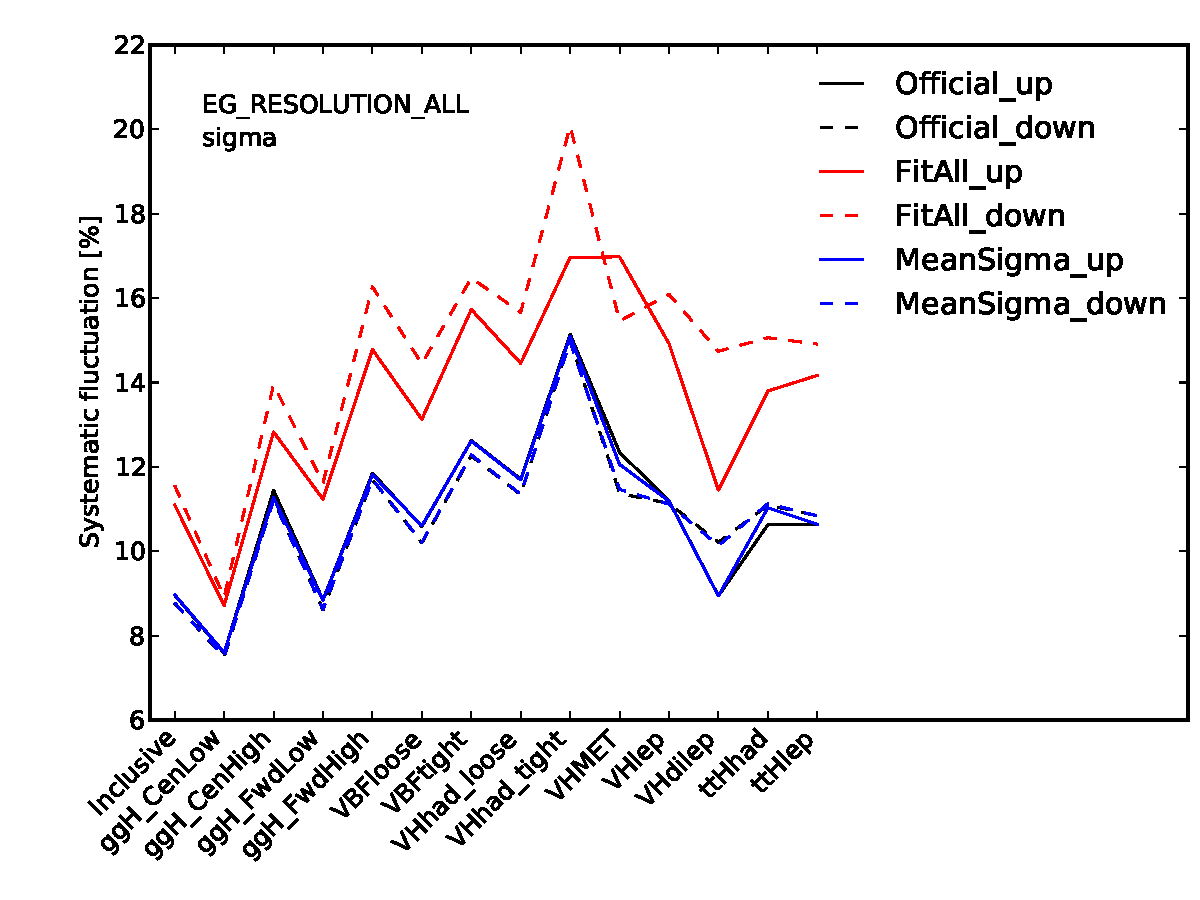
\includegraphics[width=\linewidth]{plots/Backup/h013_meanSigma_PhotonSyst_EG_RESOLUTION_ALL_sigma.pdf}\\
  \end{minipage}
  \hfill
  \begin{minipage}{0.59\linewidth}
    \begin{itemize}
    \item $\sigma$ is sensitive to the change of scale.
    \item Two understood explanations :
      \begin{itemize}
      \item $\mu /\sigma$ correlation when scaling energies.
      \item Resolution loss due to inhomogenous scaling.
        \end{itemize}
      \vfill
    \item Effect on resolution is small but I propose to \textcolor{red}{add a width effect linked to EG\_SCALE\_ALL nuisance parameter}.
      \begin{itemize}
      \item Add a second nuisance parameter to the width to limit overconstraints.
      \item Good hopes to reduce Zee resolution systematics (dominant in EG\_RESOLUTION\_ALL) within medium timescale.
      \end{itemize}
    \end{itemize}
  \end{minipage}
\end{frame}

%%=============================================================
\begin{frame}{Cross-check : template method}
\begin{minipage}{0.59\linewidth}
  The template method is used to measure $\alpha$ and $C$ simultaneously.
\begin{itemize}
\item Create distorded MC (templates) with test values of $\alpha$ and $C$.
\item \textcolor{blue}{\bf Compute $\chi^2$ between Z mass distribution of data and template}.
\item \textcolor{blue}{\bf Fit the minimum of the $\chi^2$ distribution} in the ($\alpha,C$) plane.
\item Fit performed in 2 steps of 1D fits : 
\begin{itemize}
\item fit $\chi^2=f(\alpha)$ at constant $C$ (lines) $\rightarrow (\alpha_{min}, \chi^2_{min})$ .
\item fit $\chi^2_{min}=f(C)\rightarrow (C, \Delta C)$
\item project $C$ in $\alpha_{min}=f(C)$, corresponding bin gives $(\alpha, \Delta\alpha)$.
\end{itemize}
\end{itemize}
  \includegraphics[width=0.325\linewidth]{plots/Backup/MC6_0_0_chi2FitNonConstVar_10.pdf}
  \includegraphics[width=0.325\linewidth]{plots/Backup/MC6_0_0_chi2FitConstVar.pdf}
  \includegraphics[width=0.325\linewidth]{plots/Backup/MC6_0_0_corAngle.pdf}
\end{minipage}
\hfill
\begin{minipage}{0.4\linewidth}
  \includegraphics[width=\linewidth]{plots/Backup/MC6_0_0_CompareAlpha.pdf}\\
  \includegraphics[width=\linewidth]{plots/Backup/MC6_0_0_chiMatrix.pdf}\\
\end{minipage}
\end{frame}

%==============================================================================
\begin{frame}{Scale factors interpretation}
  \begin{minipage}{0.49\linewidth}
    Assume the up fluctuation (red) as data and nominal distribution (black) as MC in the template method.
    One has
    $$m_H^{up}=m_H^{nom}(1+\alpha)$$
    Hence
    $$\delta_{m_H}=\alpha$$
    \end{minipage}
  \begin{minipage}{0.49\linewidth}
    \includegraphics[width=\linewidth]{plots/Backup/h013_EG_SCALE_ALL_0.pdf}
  \end{minipage}
  Furthermore :
  $$\sigma_H^{up}=\sigma_H^{nom} \oplus cE$$
  Hence
  $$\delta_{\sigma_H} = \sqrt{1+\frac{c^2E^2}{\sigma_H^2}}-1$$
  One has to be carefull with resolution uncertainty as the template method is weak to measure small differences.
\end{frame}

\end{document}


